\section{Silniki magazynu danych}
Architektura MySQL wspiera wiele różnych silników, które są  odpowiedzialne za wykonywanie operacji na danych. Silnik bazy danych wybierany jest per tabela, co oznacza, że w ramach pojedynczej bazy danych może być wykorzystywanych wiele różnych silników. 
\subsection{Krótka charakterystyka podstawowych silników.}
W tym podrozdziale nie będę się skupiał na szczegółowym opisie większości z silników dostępnych w MySQL, postaram się raczej w ogólny sposób przedstawić główne charakterystyki, zalety oraz ograniczenia. Część z silników została pominięta ze względu na ich marginalne użycie.
\subsubsection{MyISAM}
MyISAM jest domyślnym silnikiem składowania danych do wersji 5.4 (włącznie). W tym rozwiązaniu tabela jest przechowywana w postaci dwóch plików na dysku. Dane przechowywane są w pliku z rozszerzeniem \textbf{.MYD (MYData)}
natomiast w drugim pliku (\textbf{.MYI(MYIndex)}) przechowywane są indeksy. Poniżej przedstawię kilka cech tego silnika bazy danych. Obecnie MyISAM nie jest już rozwijany.
\begin{itemize}
	\item \textbf{Brak wsparcia dla transakcji.} Z tego powodu MyISAM nie powinien być używany do tabel, dla których istotnym wymaganiem jest zapewnienie integralności danych.
	\item \textbf{Blokada typu WRITE.}  W momencie, kiedy wykonujemy operacje dodającą dane do tabeli, jest ona blokowana na cały czas wykonywania operacji (również dla operacji odczytujących dane). Sprawia to, że w przypadku dużej liczby operacji modyfikujących dane - wydajność bazy danych wyraźnie spada.
	\item \textbf{Brak obłusgi mechanizmu kluczy obcych}
	\item \textbf{Mechanizm kompresji danych.} Silnik umożliwia kompresowanie danych w celu optymalizacji ilości miejsca potrzebnego do przechowywania danych z tabeli. Taka operacja sprawia, że "spakowane" dane są dostępne jedynie do odczytu, a ich modyfikacja jest zablokowana.	Tabele MyISAM można kompresować za pomocą mechanizmu \textit{myisampack}. 
	\item \textbf{Buforowanie indeksów.} Silnik MyISAM buforuje jedynie indeksy.
\end{itemize}

\\todo jakies podsumowanie?

\subsubsection{InnoDB}
Od wersji 5.5 InnoDB jest domyślnym silnikiem bazy danych MySQL. Mechanizm InnoDB zawiera wiele rozwiazań, których brakowało w MyISAM i obecnie jest zdecydowanie najpopularniejszym silnikiem używanym w MySQL. Domyślnie dane przechowywane są w pojedynczych plikach, ale możliwe mogą być również przechowywane w wielu plikach. Struktura plików bazy \textit{StackOverflow}, która dla wszystkich tabel używa silnika InnoDB, została przedstawiona na poniższej grafice. 
\begin{figure}[!h]
	\caption{Pliki silnika InnoDB testowej bazy danych \textit{StackOverflow}}
	\centering
	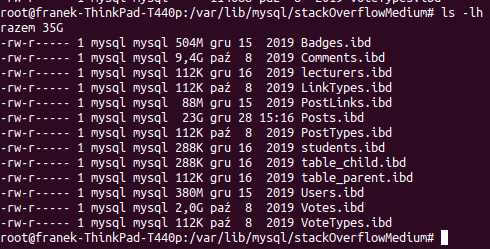
\includegraphics[scale = 0.43]{innodb-files.png}
	\label{fig:label}
\end{figure}

\begin{itemize}
	\item \textbf{Wsparcie dla transakcji. }
	\item \textbf{Blokowanie dostępu na poziomie rekordów. } Dostęp do tabel InnoDB jest blokowany za pomocą mechanizmy MVCC (Multi-Versioned Concurrency Control), który w przeciwieństwie do MyISAM blokuje pojedyncze rekordy, zamiast całej tabeli. Wprowadzenie tej zmiany znacząco zwiększyło wydajność równoległych operacji modyfikujące dane w tabeli.
	\item \textbf{Wsparcie dla kluczy obcych.}
	\item \textbf{Buforowanie danych oraz indeksów.} Silnik InnoDb może buforować nie tylko indeksy, ale również dane.
\end{itemize}

\subsubsection{CSV Storage Engine}
Silnik CSV Storage Engine przechowuje dane tabeli w plikach tekstowych w formacie csv z wartościami rozdzielonymi przecinkami.Ten silnik może być przydatny, jeżeli chcemy nasze dane przechowywać w formacie csv, ale posiada wiele ograniczeń, dlatego nie jest zalecane jego stosowanie w większości przypadków.

\begin{itemize}
	\item \textbf{Brak wsparcia dla indeksów.}
	\item \textbf{Brak możliwości przechowywania wartości \textit{null}.}
	\item \textbf{Brak wsparcia dla partycjonowania.}
\end{itemize}

\subsubsection{Memory}
Tabele z silnikiem Memory są tabelami, których dane przechowywane są w pamięci, a nie na dysku twardym. Dane przechowywane w tabeli są ulotne i zostają usunięte w momencie restartu serwera (struktura tabeli zostaje zachowana). Z powodu przechowywania w pamięci są o rząd wielkości szybsze od standardowych silników baz danych, ale ze względu na swoją ulotność nie powinny przechowywać istotnych danych dla aplikacji. Poniżej wymieniłem kilka przypadków użyca tabeli z silnikiem Memory. 
\begin{itemize}
	\item Pamięć podręczna dla często odczytywanych danych, która jest wczytywana w momencie startu serwera.
	\item Buforowanie wyników agregowanych danych z często wykonywanych zapytań.
	\item Przechowywanie wyników pośrednich z zapytań.
	\item MySQL używa tabeli Memory do wewnętrznego przetwarzania zapytań wymagających tabeli tymczasowych do przechowywania wyników pośrednich.
\end{itemize}
Niżej przedstawiłem kilka podstawowych własności tabeli Memory.
\begin{itemize}
	\item \textbf{Indeksy Hash} Tabele Memory obsługują indeksy Hash (opisane w rozdziale dotyczącym indeksów).
	\item \textbf{Blokowanie na poziomie tabeli.} Podobnie jak tabele MyISAM, w momencie modyfikowania danych blokowana jest cała tabela.
	\item \textbf{Brak obsługi typów TEXT oraz BLOB}. Tabele nie obsługują typów TEXT. Przechowywanie teksu możliwe jest w kolumnach VARCHAR o stałej zdefiniowanej wielkości, co prowadzi do marnotrawienia pamięci.
\end{itemize}


\subsubsection{Silnik Archive}
Silnik archive służącym do przechowywania dużej ilości nieindeksowanych danych, które są rzadko pobierane. 

\begin{itemize}
	\item \textbf{Możliwe wykonywanie jedynie operacji INSERT, REPLACE oraz SELECT}. W tabelach Archive niemożliwe jest usuwanie i modyfikowanie istniejących krotek.
	\item \textbf{Brak wsparcia dla indeksów.}
	\item \textbf{Blokowanie na poziomie tabeli.}
	\item \textbf{Kompresowanie danych.} Każdy wstawiony rekord jest automatycznie kompresowany za pomocą \textit{zlib}, dlatego tabele Archive wymagają zdecydowanie mniej miejsca od tabel InnoDB lub MyISAM.
	\textit{Brak wsparcia dla transakcji.}
\end{itemize}

\subsubsection{Silnik NDB Cluster}
Silnik NDB Cluster został zaprojektowany do działania w klastrze MySQL. Został opracowany w celu zapewnienia dużej szbkości działania wraz z możliwościami w zakresie redundancji i równoważenia obciążenia. Pierwotnie został zaprojektowany do przechowywania danych w pamięci, ale obecnie możliwe jest również przechowywanie danych na dysku twardym. Zastosowanie silnika NDB Cluster jest dokładniej opisane w rozdziale dotyczącym skalowania.

\subsection{Porównanie silników}
\\todo https://dev.mysql.com/doc/refman/8.0/en/storage-engines.html


W celu porównania silników baz danych przygotowałem testową bazę danych zawierają pięć tabel będących niemalże kopią tabeli \textit{Users} z bazy testowej, z których każda wykorzystuje inny silnik. Jedyną zmianą jest usunięcie kolumny \textit{AboutMe}, która została usunięta ze względu na fakt, że silnik MEMORY nie wspiera typu TEXT. Do tworzenia tabel wykorzystałem następujące polecenie.
\begin{spverbatim}
	CREATE TABLE `Users` (
	`Id` int NOT NULL,
	`Age` int NOT NULL DEFAULT 0,
	`CreationDate` datetime NOT NULL,
	`DisplayName` varchar(80) NOT NULL,
	`DownVotes` int NOT NULL,
	`EmailHash` varchar(80) NOT NULL DEFAULT '',
	`LastAccessDate` datetime NOT NULL,
	`Location` varchar(200) NOT NULL DEFAULT '',
	`Reputation` int NOT NULL,
	`UpVotes` int NOT NULL,
	`Views` int NOT NULL,
	`WebsiteUrl` varchar(400) NOT NULL DEFAULT '',
	`AccountId` int NOT NULL DEFAULT 0,
	PRIMARY KEY (`Id`) -- w tabelach, które wspierają klucze główne
	) ENGINE=<nazwa silnika>;
\end{spverbatim}
Dla silników, które nie wspierają kluczy głównych musiałem je usunąć.Dla tych, które nie wspierają przechowywania wartości NULL zamieniłem domyślne wartości NULL na wartość 0 lub pustego tekstu (w zależności od typu danych).
Tabela zawiera blisko dwa i pół miliona wierszy.
Silnik NDB pominąłem, ponieważ został dodatkowo opisany w rozdziale dotyczącym skalowalności, a jego zastosowanie jest ograniczone do specyficznych przypadków wymagających wysokiej skalowalności, dlatego jego porównanie z innymi silnikami mogło być niemiarodajne. Po stworzeniu tabel i zaimportowaniu danych, baza danych wygląda następująco.
\begin{figure}[!h]
	\caption{Baza danych użyta do testowania silników baz danych}
	\centering
	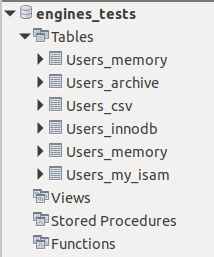
\includegraphics[scale = 0.59]{engines_tests.png}
	\label{fig:label}
\end{figure}
Do testowania zapytań wykorzystałem narzędzie \textit{mysqlslap} lub gotowe zastawy testowe narzędzia \textit{sysbench}.
\subsection{Przechowywanie danych}
\\todo rozmiar tez

\subsubsection{Wymaganie transakcyjności}
W przypadku tabel, które wymagają użycia transakcji, jedynym możliwym wyborem jest silnik InnoDB.
\subsubsection{Operacje odczytu z wykorzystaniem klucza głównego}
Aby przetestować wydajność wyszukiwania danych dla różnych silników przygotowałem następują procedurę.
\begin{spverbatim}
	create procedure test_select_users()
	begin
	declare v_max int unsigned default 20000;
	declare v_counter int unsigned default 0;
	while v_counter < v_max do
		SET @START = ROUND(RAND() * 10000);
		SELECT id, DisplayName, Reputation FROM engines_tests.Users<Nazwa_silnika> where id = @START;
		set v_counter=v_counter+1;
	end while;
	end #
\end{spverbatim}

Następnie za pomocą polecenia: \begin{spverbatim}
	mysqlslap --concurrency=10 --iterations=5 --query="call test_select_users();" --delimiter=";" --user=root --password=root --create-schema=engines_tests
\end{spverbatim} zmierzyłem wydajność pobierania 20000 losowych danych z różnych tabel i wyniki zamieściłem w poniższej tabeli.

\begin{center}
	\begin{tabular}{ | c | c | c | c | c | c |}
		\hline
		- & MyISAM & InnoDB & Memory & Archive & Csv  \\ 
		\hline
		średni czas [s] & 3.972 & 4.036 & 3.23 & powyżej 1 godziny & powyżej 1 godziny \\
		\hline
	\end{tabular}
\end{center}
Jak widzimy w przypadku zapytań wykorzystujących klucz podstawowy; trzy silniki, które posiadają taki mechanizm mają bardzo podobną wydajność. Pomiędzy testami restartowałem serwer MySQL, aby maksmymalnie wyrównać warunki. Oczywiście w mniej odizolowanym przypadku, MySQL przeprowadza pewne optymalizacje, między innymi przechowywanie często używanych danych w pamięci, co ma pewien wpływ na wydajność zapytań, ale imitując taką sytuację poprzez wielokrotne wywołanie skryptu bez restartów, wyniki nie odbiegały znacząco od tych zawartych w tabeli.

\subsubsection{Operacje odczytu bez klucza głównego}
Do przeprowadzenia testu zmodyfikowałem kluczową część procedury testującej w następujący sposób:
\begin{spverbatim}
	SET @START = ROUND(RAND() * 3000);
	SELECT id, DisplayName, Reputation FROM engines_tests.Users<Nazwa_silnika> where reputation = @START;
\end{spverbatim}
Zmodyfikowałem również liczbę zapytań do 100 (zmienna \textit{v\textunderscore max}).
